%% bare_jrnl.tex
%% V1.4b
%% 2015/08/26
%% by Michael Shell
%% see http://www.michaelshell.org/
%% for current contact information.
%%
%% This is a skeleton file demonstrating the use of IEEEtran.cls
%% (requires IEEEtran.cls version 1.8b or later) with an IEEE
%% journal paper.
%%
%% Support sites:
%% http://www.michaelshell.org/tex/ieeetran/
%% http://www.ctan.org/pkg/ieeetran
%% and
%% http://www.ieee.org/

%%*************************************************************************
%% Legal Notice:
%% This code is offered as-is without any warranty either expressed or
%% implied; without even the implied warranty of MERCHANTABILITY or
%% FITNESS FOR A PARTICULAR PURPOSE! 
%% User assumes all risk.
%% In no event shall the IEEE or any contributor to this code be liable for
%% any damages or losses, including, but not limited to, incidental,
%% consequential, or any other damages, resulting from the use or misuse
%% of any information contained here.
%%
%% All comments are the opinions of their respective authors and are not
%% necessarily endorsed by the IEEE.
%%
%% This work is distributed under the LaTeX Project Public License (LPPL)
%% ( http://www.latex-project.org/ ) version 1.3, and may be freely used,
%% distributed and modified. A copy of the LPPL, version 1.3, is included
%% in the base LaTeX documentation of all distributions of LaTeX released
%% 2003/12/01 or later.
%% Retain all contribution notices and credits.
%% ** Modified files should be clearly indicated as such, including  **
%% ** renaming them and changing author support contact information. **
%%*************************************************************************


% *** Authors should verify (and, if needed, correct) their LaTeX system  ***
% *** with the testflow diagnostic prior to trusting their LaTeX platform ***
% *** with production work. The IEEE's font choices and paper sizes can   ***
% *** trigger bugs that do not appear when using other class files.       ***                          ***
% The testflow support page is at:
% http://www.michaelshell.org/tex/testflow/



\documentclass[journal]{IEEEtran}
%
\usepackage{graphicx}
\usepackage{amsmath}
\usepackage{subcaption}
% If IEEEtran.cls has not been installed into the LaTeX system files,
% manually specify the path to it like:
% \documentclass[journal]{../sty/IEEEtran}

\usepackage{tikz}
\usetikzlibrary{positioning,arrows.meta,calc}



% Some very useful LaTeX packages include:
% (uncomment the ones you want to load)


% *** MISC UTILITY PACKAGES ***
%
%\usepackage{ifpdf}
% Heiko Oberdiek's ifpdf.sty is very useful if you need conditional
% compilation based on whether the output is pdf or dvi.
% usage:
% \ifpdf
%   % pdf code
% \else
%   % dvi code
% \fi
% The latest version of ifpdf.sty can be obtained from:
% http://www.ctan.org/pkg/ifpdf
% Also, note that IEEEtran.cls V1.7 and later provides a builtin
% \ifCLASSINFOpdf conditional that works the same way.
% When switching from latex to pdflatex and vice-versa, the compiler may
% have to be run twice to clear warning/error messages.






% *** CITATION PACKAGES ***
%
%\usepackage{cite}
% cite.sty was written by Donald Arseneau
% V1.6 and later of IEEEtran pre-defines the format of the cite.sty package
% \cite{} output to follow that of the IEEE. Loading the cite package will
% result in citation numbers being automatically sorted and properly
% "compressed/ranged". e.g., [1], [9], [2], [7], [5], [6] without using
% cite.sty will become [1], [2], [5]--[7], [9] using cite.sty. cite.sty's
% \cite will automatically add leading space, if needed. Use cite.sty's
% noadjust option (cite.sty V3.8 and later) if you want to turn this off
% such as if a citation ever needs to be enclosed in parenthesis.
% cite.sty is already installed on most LaTeX systems. Be sure and use
% version 5.0 (2009-03-20) and later if using hyperref.sty.
% The latest version can be obtained at:
% http://www.ctan.org/pkg/cite
% The documentation is contained in the cite.sty file itself.






% *** GRAPHICS RELATED PACKAGES ***
%
\ifCLASSINFOpdf
  % \usepackage[pdftex]{graphicx}
  % declare the path(s) where your graphic files are
  % \graphicspath{{../pdf/}{../jpeg/}}
  % and their extensions so you won't have to specify these with
  % every instance of \includegraphics
  % \DeclareGraphicsExtensions{.pdf,.jpeg,.png}
\else
  % or other class option (dvipsone, dvipdf, if not using dvips). graphicx
  % will default to the driver specified in the system graphics.cfg if no
  % driver is specified.
  % \usepackage[dvips]{graphicx}
  % declare the path(s) where your graphic files are
  % \graphicspath{{../eps/}}
  % and their extensions so you won't have to specify these with
  % every instance of \includegraphics
  % \DeclareGraphicsExtensions{.eps}
\fi
% graphicx was written by David Carlisle and Sebastian Rahtz. It is
% required if you want graphics, photos, etc. graphicx.sty is already
% installed on most LaTeX systems. The latest version and documentation
% can be obtained at: 
% http://www.ctan.org/pkg/graphicx
% Another good source of documentation is "Using Imported Graphics in
% LaTeX2e" by Keith Reckdahl which can be found at:
% http://www.ctan.org/pkg/epslatex
%
% latex, and pdflatex in dvi mode, support graphics in encapsulated
% postscript (.eps) format. pdflatex in pdf mode supports graphics
% in .pdf, .jpeg, .png and .mps (metapost) formats. Users should ensure
% that all non-photo figures use a vector format (.eps, .pdf, .mps) and
% not a bitmapped formats (.jpeg, .png). The IEEE frowns on bitmapped formats
% which can result in "jaggedy"/blurry rendering of lines and letters as
% well as large increases in file sizes.
%
% You can find documentation about the pdfTeX application at:
% http://www.tug.org/applications/pdftex





% *** MATH PACKAGES ***
%
%\usepackage{amsmath}
% A popular package from the American Mathematical Society that provides
% many useful and powerful commands for dealing with mathematics.
%
% Note that the amsmath package sets \interdisplaylinepenalty to 10000
% thus preventing page breaks from occurring within multiline equations. Use:
%\interdisplaylinepenalty=2500
% after loading amsmath to restore such page breaks as IEEEtran.cls normally
% does. amsmath.sty is already installed on most LaTeX systems. The latest
% version and documentation can be obtained at:
% http://www.ctan.org/pkg/amsmath





% *** SPECIALIZED LIST PACKAGES ***
%
%\usepackage{algorithmic}
% algorithmic.sty was written by Peter Williams and Rogerio Brito.
% This package provides an algorithmic environment fo describing algorithms.
% You can use the algorithmic environment in-text or within a figure
% environment to provide for a floating algorithm. Do NOT use the algorithm
% floating environment provided by algorithm.sty (by the same authors) or
% algorithm2e.sty (by Christophe Fiorio) as the IEEE does not use dedicated
% algorithm float types and packages that provide these will not provide
% correct IEEE style captions. The latest version and documentation of
% algorithmic.sty can be obtained at:
% http://www.ctan.org/pkg/algorithms
% Also of interest may be the (relatively newer and more customizable)
% algorithmicx.sty package by Szasz Janos:
% http://www.ctan.org/pkg/algorithmicx




% *** ALIGNMENT PACKAGES ***
%
%\usepackage{array}
% Frank Mittelbach's and David Carlisle's array.sty patches and improves
% the standard LaTeX2e array and tabular environments to provide better
% appearance and additional user controls. As the default LaTeX2e table
% generation code is lacking to the point of almost being broken with
% respect to the quality of the end results, all users are strongly
% advised to use an enhanced (at the very least that provided by array.sty)
% set of table tools. array.sty is already installed on most systems. The
% latest version and documentation can be obtained at:
% http://www.ctan.org/pkg/array


% IEEEtran contains the IEEEeqnarray family of commands that can be used to
% generate multiline equations as well as matrices, tables, etc., of high
% quality.




% *** SUBFIGURE PACKAGES ***
%\ifCLASSOPTIONcompsoc
%  \usepackage[caption=false,font=normalsize,labelfont=sf,textfont=sf]{subfig}
%\else
%  \usepackage[caption=false,font=footnotesize]{subfig}
%\fi
% subfig.sty, written by Steven Douglas Cochran, is the modern replacement
% for subfigure.sty, the latter of which is no longer maintained and is
% incompatible with some LaTeX packages including fixltx2e. However,
% subfig.sty requires and automatically loads Axel Sommerfeldt's caption.sty
% which will override IEEEtran.cls' handling of captions and this will result
% in non-IEEE style figure/table captions. To prevent this problem, be sure
% and invoke subfig.sty's "caption=false" package option (available since
% subfig.sty version 1.3, 2005/06/28) as this is will preserve IEEEtran.cls
% handling of captions.
% Note that the Computer Society format requires a larger sans serif font
% than the serif footnote size font used in traditional IEEE formatting
% and thus the need to invoke different subfig.sty package options depending
% on whether compsoc mode has been enabled.
%
% The latest version and documentation of subfig.sty can be obtained at:
% http://www.ctan.org/pkg/subfig




% *** FLOAT PACKAGES ***
%
%\usepackage{fixltx2e}
% fixltx2e, the successor to the earlier fix2col.sty, was written by
% Frank Mittelbach and David Carlisle. This package corrects a few problems
% in the LaTeX2e kernel, the most notable of which is that in current
% LaTeX2e releases, the ordering of single and double column floats is not
% guaranteed to be preserved. Thus, an unpatched LaTeX2e can allow a
% single column figure to be placed prior to an earlier double column
% figure.
% Be aware that LaTeX2e kernels dated 2015 and later have fixltx2e.sty's
% corrections already built into the system in which case a warning will
% be issued if an attempt is made to load fixltx2e.sty as it is no longer
% needed.
% The latest version and documentation can be found at:
% http://www.ctan.org/pkg/fixltx2e


%\usepackage{stfloats}
% stfloats.sty was written by Sigitas Tolusis. This package gives LaTeX2e
% the ability to do double column floats at the bottom of the page as well
% as the top. (e.g., "\begin{figure*}[!b]" is not normally possible in
% LaTeX2e). It also provides a command:
%\fnbelowfloat
% to enable the placement of footnotes below bottom floats (the standard
% LaTeX2e kernel puts them above bottom floats). This is an invasive package
% which rewrites many portions of the LaTeX2e float routines. It may not work
% with other packages that modify the LaTeX2e float routines. The latest
% version and documentation can be obtained at:
% http://www.ctan.org/pkg/stfloats
% Do not use the stfloats baselinefloat ability as the IEEE does not allow
% \baselineskip to stretch. Authors submitting work to the IEEE should note
% that the IEEE rarely uses double column equations and that authors should try
% to avoid such use. Do not be tempted to use the cuted.sty or midfloat.sty
% packages (also by Sigitas Tolusis) as the IEEE does not format its papers in
% such ways.
% Do not attempt to use stfloats with fixltx2e as they are incompatible.
% Instead, use Morten Hogholm'a dblfloatfix which combines the features
% of both fixltx2e and stfloats:
%
% \usepackage{dblfloatfix}
% The latest version can be found at:
% http://www.ctan.org/pkg/dblfloatfix




%\ifCLASSOPTIONcaptionsoff
%  \usepackage[nomarkers]{endfloat}
% \let\MYoriglatexcaption\caption
% \renewcommand{\caption}[2][\relax]{\MYoriglatexcaption[#2]{#2}}
%\fi
% endfloat.sty was written by James Darrell McCauley, Jeff Goldberg and 
% Axel Sommerfeldt. This package may be useful when used in conjunction with 
% IEEEtran.cls'  captionsoff option. Some IEEE journals/societies require that
% submissions have lists of figures/tables at the end of the paper and that
% figures/tables without any captions are placed on a page by themselves at
% the end of the document. If needed, the draftcls IEEEtran class option or
% \CLASSINPUTbaselinestretch interface can be used to increase the line
% spacing as well. Be sure and use the nomarkers option of endfloat to
% prevent endfloat from "marking" where the figures would have been placed
% in the text. The two hack lines of code above are a slight modification of
% that suggested by in the endfloat docs (section 8.4.1) to ensure that
% the full captions always appear in the list of figures/tables - even if
% the user used the short optional argument of \caption[]{}.
% IEEE papers do not typically make use of \caption[]'s optional argument,
% so this should not be an issue. A similar trick can be used to disable
% captions of packages such as subfig.sty that lack options to turn off
% the subcaptions:
% For subfig.sty:
% \let\MYorigsubfloat\subfloat
% \renewcommand{\subfloat}[2][\relax]{\MYorigsubfloat[]{#2}}
% However, the above trick will not work if both optional arguments of
% the \subfloat command are used. Furthermore, there needs to be a
% description of each subfigure *somewhere* and endfloat does not add
% subfigure captions to its list of figures. Thus, the best approach is to
% avoid the use of subfigure captions (many IEEE journals avoid them anyway)
% and instead reference/explain all the subfigures within the main caption.
% The latest version of endfloat.sty and its documentation can obtained at:
% http://www.ctan.org/pkg/endfloat
%
% The IEEEtran \ifCLASSOPTIONcaptionsoff conditional can also be used
% later in the document, say, to conditionally put the References on a 
% page by themselves.




% *** PDF, URL AND HYPERLINK PACKAGES ***
%
%\usepackage{url}
% url.sty was written by Donald Arseneau. It provides better support for
% handling and breaking URLs. url.sty is already installed on most LaTeX
% systems. The latest version and documentation can be obtained at:
% http://www.ctan.org/pkg/url
% Basically, \url{my_url_here}.




% *** Do not adjust lengths that control margins, column widths, etc. ***
% *** Do not use packages that alter fonts (such as pslatex).         ***
% There should be no need to do such things with IEEEtran.cls V1.6 and later.
% (Unless specifically asked to do so by the journal or conference you plan
% to submit to, of course. )


% correct bad hyphenation here
\hyphenation{op-tical net-works semi-conduc-tor}


\begin{document}
%
% paper title
% Titles are generally capitalized except for words such as a, an, and, as,
% at, but, by, for, in, nor, of, on, or, the, to and up, which are usually
% not capitalized unless they are the first or last word of the title.
% Linebreaks \\ can be used within to get better formatting as desired.
% Do not put math or special symbols in the title.

% paper title
\title{
  \hfill\parbox{\textwidth}{\raggedleft
    \normalsize Proceedings of the 2026 \\
    International Symposium on Flexible Automation \\
    ISFA2026 \\
    July 19-22, 2026, Okayama, Japan \\[10pt]
    \Large \textbf{ISFA2026-XXXXXX}
  }\\[2em] % Adds spacing between the header and the actual title
  A Virtual-Dynamics Admittance Framework for Perception-Driven Orientation Control in Robotic Inspection
}
%
%
% author names and IEEE memberships
% note positions of commas and nonbreaking spaces ( ~ ) LaTeX will not break
% a structure at a ~ so this keeps an author's name from being broken across
% two lines.
% use \thanks{} to gain access to the first footnote area
% a separate \thanks must be used for each paragraph as LaTeX2e's \thanks
% was not built to handle multiple paragraphs
%

\author{Antara~Banerjee*,
        Colin~Acton*,
        and~Xu~Chen% <-this % stops a space
\thanks{Antara Banerjee is with the Department
of Electrical and Computer Engineering, and Colin Acton and Xu Chen are with the Department of Mechanical Engineering, University of Washington, Seattle.}% <-this % stops a space
\thanks{* denotes equal contribution.}}

% note the % following the last \IEEEmembership and also \thanks - 
% these prevent an unwanted space from occurring between the last author name
% and the end of the author line. i.e., if you had this:
% 
% \author{....lastname \thanks{...} \thanks{...} }
%                     ^------------^------------^----Do not want these spaces!
%
% a space would be appended to the last name and could cause every name on that
% line to be shifted left slightly. This is one of those "LaTeX things". For
% instance, "\textbf{A} \textbf{B}" will typeset as "A B" not "AB". To get
% "AB" then you have to do: "\textbf{A}\textbf{B}"
% \thanks is no different in this regard, so shield the last } of each \thanks
% that ends a line with a % and do not let a space in before the next \thanks.
% Spaces after \IEEEmembership other than the last one are OK (and needed) as
% you are supposed to have spaces between the names. For what it is worth,
% this is a minor point as most people would not even notice if the said evil
% space somehow managed to creep in.



% The paper headers
% \markboth{Journal of \LaTeX\ Class Files,~Vol.~14, No.~8, August~2015}%
% {Shell \MakeLowercase{\textit{et al.}}: Perception-Driven Compliant Orientation Control Using Virtual-Dynamics Admittance Modeling}


% The only time the second header will appear is for the odd numbered pages
% after the title page when using the twoside option.
% 
% *** Note that you probably will NOT want to include the author's ***
% *** name in the headers of peer review papers.                   ***
% You can use \ifCLASSOPTIONpeerreview for conditional compilation here if
% you desire.




% If you want to put a publisher's ID mark on the page you can do it like
% this:
%\IEEEpubid{0000--0000/00\$00.00~\copyright~2015 IEEE}
% Remember, if you use this you must call \IEEEpubidadjcol in the second
% column for its text to clear the IEEEpubid mark.



% use for special paper notices
%\IEEEspecialpapernotice{(Invited Paper)}




% make the title area
\maketitle

% As a general rule, do not put math, special symbols or citations
% in the abstract or keywords.
\begin{abstract}
Robotic visual inspection requires accurate alignment between the end-effector and local surface geometry while remaining robust to perception noise and surface irregularities. In industrial inspection tasks, a human operator is often kept in the loop to guide the robot through teleoperation or shared autonomy. Because the operator may adjust the robot motion in real time, offline motion planning alone becomes insufficient, motivating control architectures that support reactive, compliant interaction with uncertain surfaces. Traditional trajectory-based approaches rely on pre-planned motions and often struggle to adapt to such variations during execution. Additionally, when a human operator is in the loop, such approaches may generate motions that oppose user input, complicating intuitive teleoperation and manual guidance. This paper presents an admittance-based orientation control framework for perception-driven robotic inspection. The method models the manipulator end-effector as a virtual sphere moving in a viscous medium, forming a physically interpretable mass–damper system that generates compliant motion from orientation error.

Surface normals estimated from depth point clouds provide real-time orientation feedback, which is regulated using a PD controller to produce a virtual control torque about a pivot point on the surface in front of the camera. Through Newton–Euler dynamics and viscous drag modeling, this torque drives an admittance model whose integrated response generates task-space velocity commands. These velocities are converted through inverse kinematics into joint velocity commands, which are then executed by the robot controller. Experiments on a UR5e manipulator demonstrate stable orientation regulation under perception uncertainty. The proposed framework enables modular integration of perception-driven control with existing robot servo architectures, while its task-space formulation allows it to be readily applied to a wide range of robotic manipulators.

\end{abstract}

% Note that keywords are not normally used for peerreview papers.
\begin{IEEEkeywords}
Admittance control, robotic visual inspection, perception-driven control, orientation regulation, compliant control 
\end{IEEEkeywords}






% For peer review papers, you can put extra information on the cover
% page as needed:
% \ifCLASSOPTIONpeerreview
% \begin{center} \bfseries EDICS Category: 3-BBND \end{center}
% \fi
%
% For peerreview papers, this IEEEtran command inserts a page break and
% creates the second title. It will be ignored for other modes.
\IEEEpeerreviewmaketitle


\section{Introduction}
Human-robot collaborations, such as collaborative robotic assembly and inspection, require controllers that regulate the dynamic relationship between the motion of the end-effector and the interaction forces.
However, traditional industrial manipulators are primarily designed for precise position tracking and, therefore, struggle to perform tasks involving sustained physical interaction with uncertain environments. 
Early work on robotic interaction control focused on modifying robot motion based on measured forces during contact. Whitney introduced the concept of \emph{accommodation control}, where force feedback is used to modify the commanded motion of the manipulator in order to achieve stable contact during fine-motion tasks \cite{Whitney1977}. 
Raibert and Craig proposed the framework of \emph{hybrid position/force control}, which separates the control problem into motion-controlled and force-controlled directions \cite{RaibertCraig1981}. 
Hogan later formalized the concept of \emph{impedance control}, which regulates the dynamic relationship between force and motion by imposing a desired mechanical impedance at the robot end-effector \cite{Hogan1985}. In this framework, the robot behaves as a virtual mass–spring–damper system that determines how motion responds to applied forces, enabling compliant interaction with uncertain environments.

While impedance control provides a powerful dynamic interaction framework, many industrial robotic systems are position-controlled and do not provide direct torque control at the actuator level. As a result, interaction control is often implemented through outer-loop controllers that modify position or velocity commands based on measured forces. % Early experimental work by Maples and Becker demonstrated the feasibility of force control on robotic manipulators and highlighted practical considerations when implementing interaction control on position-controlled robots \cite{Maples1986}. 
% Subsequent studies analyzed the achievable accuracy of such implementations and showed that the realized impedance behavior depends strongly on factors such as inner-loop bandwidth, sampling delays, and force feedforward compensation.
Position-based impedance control, also known as 
%In response to these limitations, 
\emph{admittance control}, has then become a widely adopted approach for interaction control. In admittance control, measured interaction forces are mapped to desired motion commands through a virtual dynamic model, allowing compliant behavior to be implemented using position or velocity-controlled manipulators. Newman analyzed the stability and performance limits of interaction controllers \cite{Newman1992}.
% and demonstrated that passivity constraints impose fundamental bounds on the achievable driving-point admittance during physical interaction.
%Beyond such fundamental analysis, admittance control has also been investigated in practical manipulation tasks. 
Schimmels and Peshkin studied the robustness of an admittance control law for force-guided assembly and showed that force-to-motion mappings can be designed to remain effective even in the presence of contact friction disturbances \cite{Peshkin1992}.

Admittance control has been widely adopted in applications involving physical human--robot interaction and haptic interfaces, where the interaction force measured at the robot end-effector is used to generate motion commands through a virtual dynamic model. In this framework, a desired mass--spring--damper behavior is imposed such that the measured external force determines the commanded velocity or position of the robot. Keemink et al.~\cite{Keemink2018} provide a comprehensive overview of admittance control, clarifying its relationship with impedance control and reviewing its applications in haptic devices, rehabilitation systems, and collaborative robots. \\ 
%The authors further highlight important design challenges, particularly the trade-off between achieving low apparent inertia for transparency and maintaining stable interaction when the robot is coupled with stiff environments or human operators.\\
% Interaction stability is further influenced by implementation effects such as sampling, sensing, and computation delays. 
% Adams and Hannaford investigated the stability of admittance-based haptic control systems and showed that discrete-time implementations can become unstable when interacting with humans or environments if the virtual dynamics are not properly designed \cite{Adams1999}. Their analysis demonstrated that admittance controllers must incorporate sufficient virtual damping and compliance in order to maintain passive and stable interaction behavior. These results provide important design guidelines for admittance control systems operating in contact with uncertain environments.\\
Interaction control has also been extended to human–robot cooperation scenarios, where variable impedance and admittance controllers enable robots to adapt their dynamic behavior in response to human interaction forces. Duchaine and Gosselin proposed a velocity-based variable impedance framework that allows robots to adjust their interaction behavior during cooperative manipulation tasks \cite{Duchaine2007}.



Beyond manipulation tasks such as assembly and cooperation, interaction control is increasingly being integrated with perception-driven robotic systems. One important application is robotic visual inspection in aerospace manufacturing, where small surface defects must be detected reliably across complex geometries. Automated inspection systems that combine robotics, perception, and intelligent planning have recently been proposed to address these challenges. For example, an agile inspection framework based on unsupervised machine learning was developed to generate inspection viewpoints across complex aerospace component geometries using robotic imaging systems \cite{Nandagopal2024}. However, practical inspection tasks often require the robot to maintain close proximity  with curved and irregular surfaces, while remaining robust to perception noise and geometric uncertainty. In addition, many inspection systems operate in a human-in-the-loop setting where operators guide the robot during the inspection process, making purely pre-planned motion strategies difficult to apply. These requirements motivate the use of interaction control strategies that enable compliant and responsive robot motion during perception-driven tasks.

Motivated by these developments, this work investigates a perception-driven admittance control framework for robotic visual inspection tasks. The proposed approach integrates force-based interaction control with perception-based orientation regulation to enable compliant robot motion during human-in-the-loop inspection. The system combines a vision-based orientation controller that aligns the end-effector with estimated surface normals and an admittance controller that converts measured interaction forces into velocity commands for a collaborative manipulator. This integration enables stable and responsive robot–environment interaction while maintaining robustness to sensing noise and environmental uncertainty. While the focus of this work is robotic visual inspection, the proposed control framework is broadly applicable to other tasks involving perception-driven compliant interaction, such as surface following, polishing, or contact-based manipulation.



% needed in second column of first page if using \IEEEpubid
%\IEEEpubidadjcol
\section{Materials and Methods}
\subsection{System Architecture and Control Pipeline}
\begin{figure}[t]
    \centering
    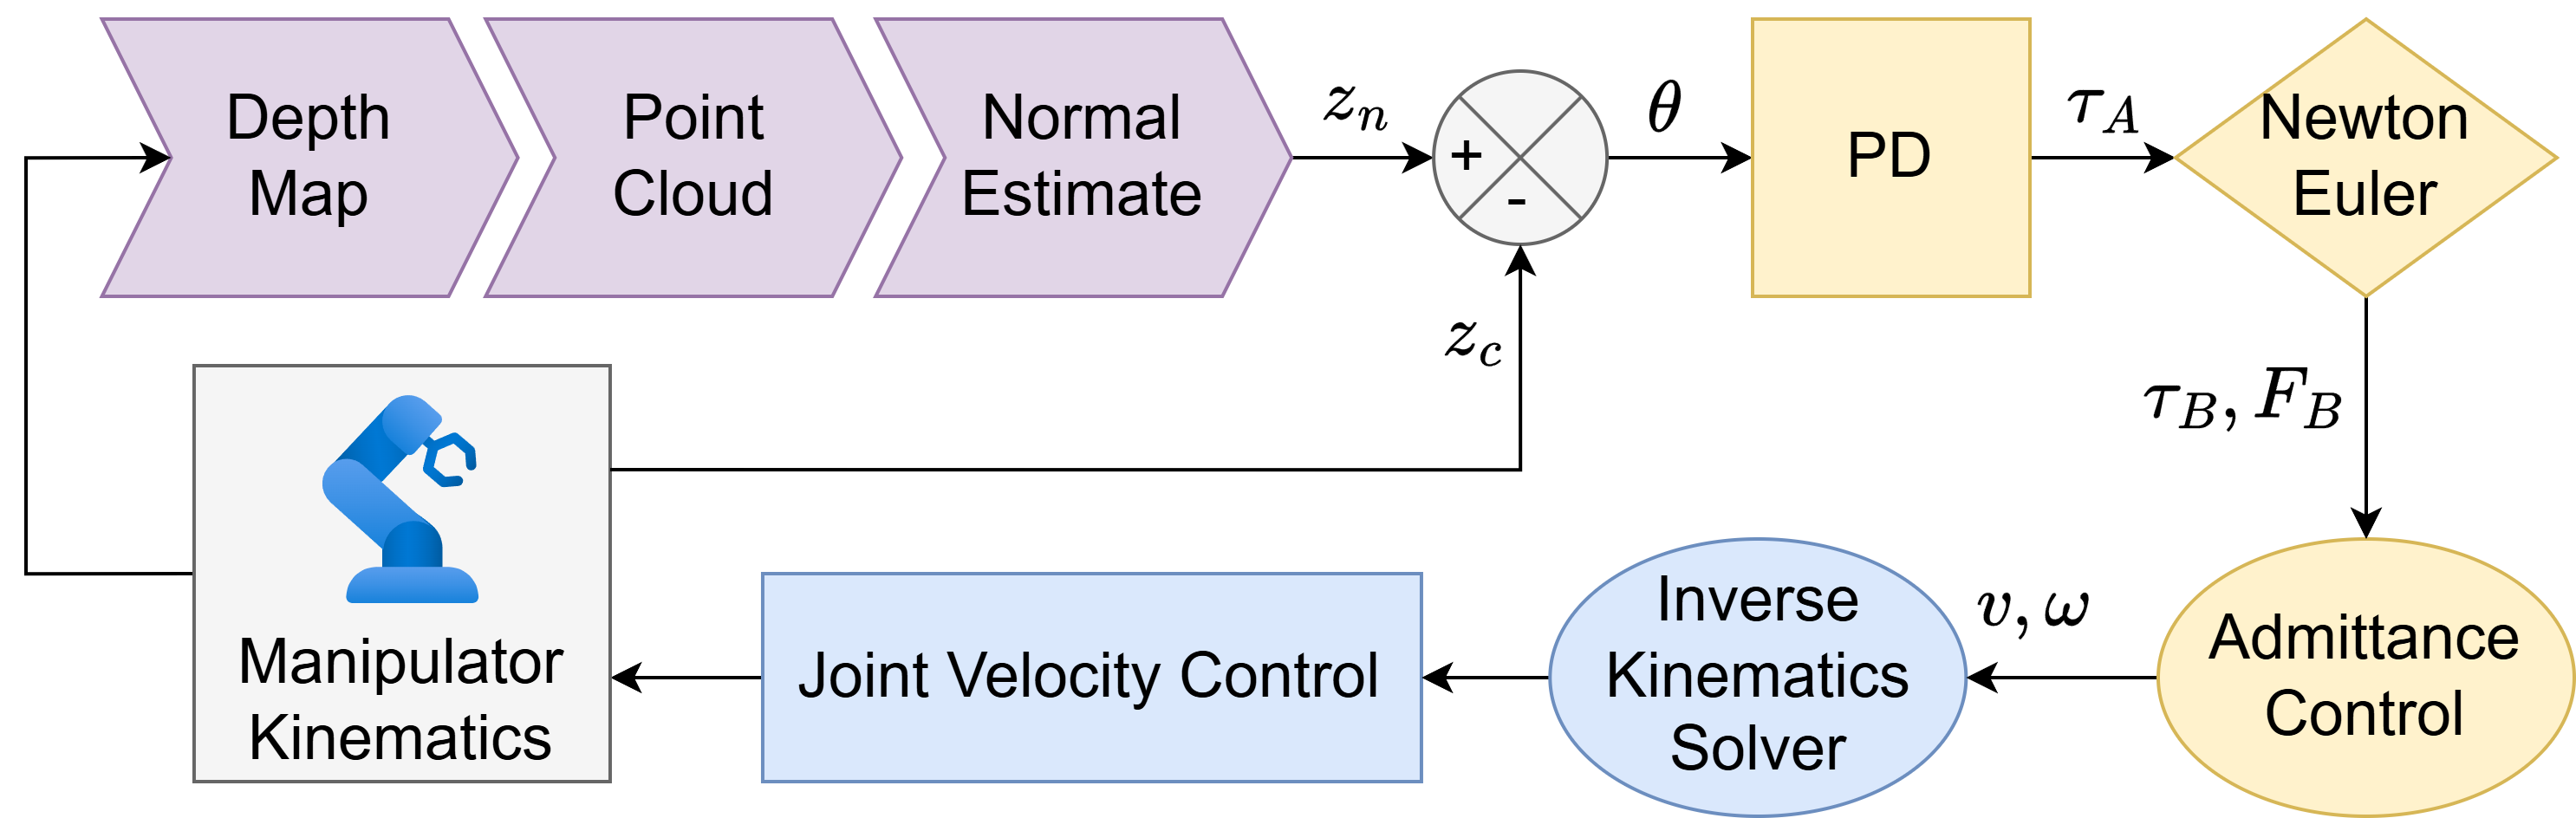
\includegraphics[width=\linewidth]{flowchartorientation.png}
    \caption{System architecture of the proposed perception-driven orientation control framework. Depth images from the Intel RealSense D405 camera are converted into point clouds and processed through filtering, downsampling, and outlier removal. Surface normals are estimated using PCA and RANSAC-based plane fitting. The resulting orientation error is converted to a PD control law which drives the admittance control node, which generates compliant motion commands. These commands are executed through the ROS~2 Servo node and forwarded to the robot controller for motion execution.}
    \label{fig:architecture}
\end{figure}
The overall architecture of the proposed inspection system integrates perception, control, and motion execution within a modular pipeline, as illustrated in Fig.~\ref{fig:architecture}. The system is implemented on a UR5e industrial manipulator equipped with an eye-in-hand Intel RealSense D405 depth camera mounted at the end-effector. The camera provides high-resolution depth measurements of the local inspection surface, enabling real-time estimation of surface geometry.

The perception pipeline begins by acquiring depth images from the RealSense D405 camera. These depth images are converted into point clouds using the camera intrinsic calibration parameters. From the resulting point cloud, a local neighborhood corresponding to the inspection region is extracted and used to estimate the surface normal of the observed surface.

Surface normal estimation is performed using a combination of   RANSAC-based plane fitting \cite{fischler1981random} and principal component analysis (PCA) \cite{winn20238}. First, the Random Sample Consensus (RANSAC) algorithm is used to robustly identify planar inliers within the point cloud while rejecting outliers caused by sensor noise or spurious depth measurements. This step ensures that the normal estimation process is not significantly affected by outliers or irregular surface points.

Once a consistent set of inlier points is identified, PCA is applied to compute the local surface normal. Given a set of $N$ points $\{\mathbf{p}_i\}$ belonging to the detected plane, the centroid of the point set is computed as

\begin{equation}
\mathbf{p}_c = \frac{1}{N} \sum_{i=1}^{N} \mathbf{p}_i.
\end{equation}

The covariance matrix of the centered points is then constructed as

\begin{equation}
C = \frac{1}{N} \sum_{i=1}^{N} (\mathbf{p}_i - \mathbf{p}_c)(\mathbf{p}_i - \mathbf{p}_c)^T.
\end{equation}

The eigenvector corresponding to the smallest eigenvalue of the covariance matrix represents the estimated surface normal direction. This normal vector defines the desired orientation for the robot end-effector during inspection.

The estimated surface normal is then compared with the current end-effector orientation to compute the orientation error. 
%This error is expressed in terms of pitch and yaw deviations between the tool axis and the desired surface normal direction.

The orientation error is processed by the outer-loop controller, implemented as a PD controller that generates a virtual control torque. This torque drives the virtual sphere dynamic model described in Section C, producing angular acceleration that reflects the desired correction motion.

The resulting angular acceleration is subsequently used to compute torque and force exerted at the end effector using Newton Euler Theorem. These force and torque are passed into the admittance model and are converted into Cartesian velocity commands in the robot task space.

The velocity commands are transmitted to the robot through the ROS~2 Servo node, which acts as the execution layer of the control architecture. The Servo node converts the task-space velocity commands into joint-level commands using the robot Jacobian and forwards them to the robot's internal controllers.

Because the ROS~2 Servo interface operates on top of the robot's existing joint servo loops, the proposed controller functions as an outer-loop compliance layer. This design allows perception-driven orientation regulation to be implemented without modifying the underlying robot control architecture, making the framework compatible with standard industrial robotic platforms.
\subsection{Admittance-Based Control Framework}

The proposed control architecture follows an admittance-based formulation in which force and torque inputs are transformed into compliant motion commands. The objective is to generate smooth and physically interpretable velocity commands for the robot end-effector while respecting actuator and servo constraints.

To provide physical intuition, the end-effector is modeled as a virtual sphere of mass $m$ and radius $R$ moving in a viscous medium characterized by dynamic viscosity $\mu$, as illustrated in Fig.~\ref{fig:virtual_mass_damper}. The inertia of the sphere about its center of mass at point $B$ is given by
\begin{equation}
I_B = \frac{2}{5} m R^2.
\end{equation}
\begin{figure}[t]
\centering
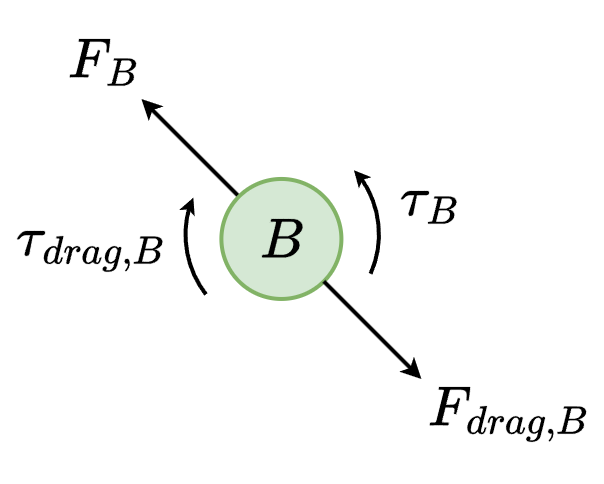
\includegraphics[width=0.45\linewidth]{admittance_massdamper.png}
\caption{Virtual mass--damper representation of the end-effector. The virtual sphere at point $B$ is subjected to equivalent force $F_B$ and torque $\tau_B$, while viscous drag $F_{\mathrm{drag},B}$ and $\tau_{\mathrm{drag},B}$ oppose motion.}
\label{fig:virtual_mass_damper}
\end{figure}
The objective of this abstraction is not to reproduce the exact rigid-body
dynamics of the manipulator, but rather to construct a virtual
dynamic model that can be used to generate compliant motion
commands for orientation and teleoperation regulation.
The viscous interaction between the virtual sphere and the surrounding medium is modeled using translational and rotational drag forces. The translational drag force acting on the sphere is given by

\begin{equation}
F_{\mathrm{drag},B} = -c_d v_B,
\end{equation}

where the drag coefficient is defined as

\begin{equation}
c_d = 6\pi \mu R.
\end{equation}

Similarly, the rotational drag torque is modeled as

\begin{equation}
\tau_{\mathrm{drag},B} = -\gamma \omega_B.
\end{equation}

While the classical Stokes rotational drag coefficient for a sphere is $8\pi \mu R^3$, a modified coefficient is used in this work:

\begin{equation}
\gamma = 2.4\pi \mu R^3.
\end{equation}

This value is approximately $3.3$ times smaller than the classical Stokes rotational drag coefficient ($8\pi\mu R^3$), and is selected to ensure synchronized translational and rotational responses of the virtual sphere as it reaches terminal rotational and linear velocities.

Using these definitions, the net inputs to the admittance model are expressed as

\begin{equation}
F_{\mathrm{net}} = F_B - c_d v_B
\end{equation}

\begin{equation}
\tau_{\mathrm{net}} = \tau_B - \gamma \omega_B.
\end{equation}
The translational and rotational admittance dynamics are defined as

\begin{equation}
m \dot{v}_B = F_{\mathrm{net}}
\end{equation}

\begin{equation}
I_B \dot{\omega}_B = \tau_{\mathrm{net}}.
\end{equation}

The resulting accelerations are integrated to obtain the commanded velocities

\begin{equation}
v_B = \int \dot{v}_B \, dt, 
\qquad 
\omega_B = \int \dot{\omega}_B \, dt.
\end{equation}

These velocities are transmitted to the robot through the ROS~2 Servo node, allowing the orientation controller to act as a compliant outer-loop layer.
\subsection{Orientation Control}

To generate the force and torque inputs required by the admittance model, a virtual rigid-body interpretation of the end-effector is introduced. The goal of this model is not to capture the full manipulator dynamics, but to provide a physically consistent mapping from orientation error to equivalent forces and torques.

As illustrated in Fig.~\ref{fig:fbd_AB}, let point $A$ denote the pivot associated with the local surface-normal frame, and let point $B$ denote the center of the virtual sphere located at a distance $d$ from point $A$. The control torque $\tau_A$ is applied at point $A$, which induces rotational motion of the virtual sphere.

\begin{figure}[t]
\centering
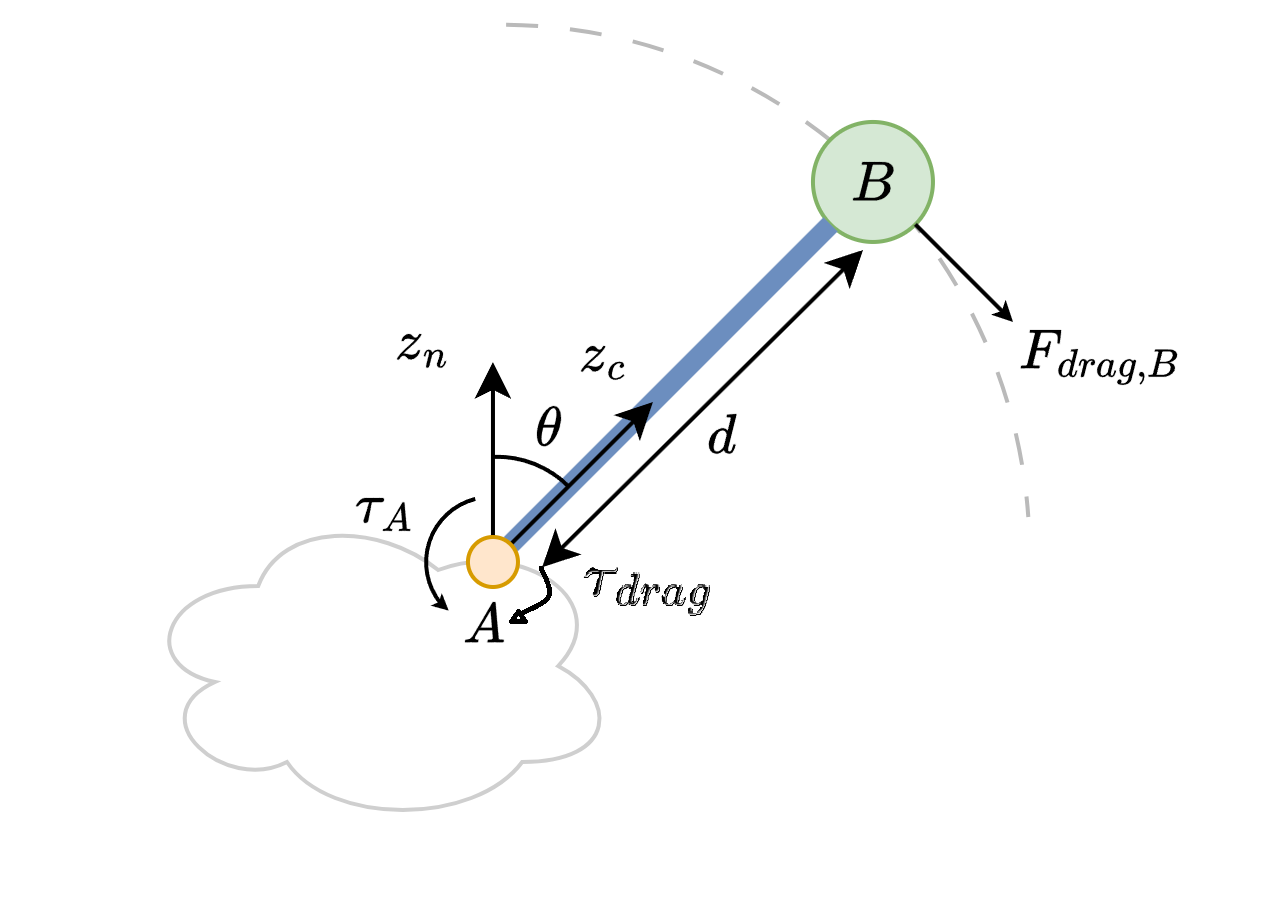
\includegraphics[width=0.7\linewidth]{Rigid_body.png}
\caption{Rigid-body interpretation of the virtual sphere. Point $A$ represents the pivot where control torque $\tau_A$ is applied, and point $B$ denotes the center of mass of the virtual sphere located at a distance $d$.}
\label{fig:fbd_AB}
\end{figure}

\subsubsection{Rotational dynamics about pivot}

The applied torque $\tau_A$ produces angular acceleration $\alpha = \ddot{\theta}$ about point $A$. The inertia about the pivot is obtained using the parallel-axis theorem:

\begin{equation}
I_A = I_B + md^2
\end{equation}

where $I_B = \frac{2}{5} m R^2$ is the inertia of the virtual sphere about its center of mass.

The rotational dynamics about point $A$ are given by

\begin{equation}
\tau_A = I_A \alpha - \tau_{\mathrm{drag}}.
\end{equation}

\subsubsection{Viscous drag torque}

The translational drag force acting on the sphere is modeled using Stokes drag:

\begin{equation}
F_{\mathrm{drag},B} = -6\pi \mu R v_B
\end{equation}

where $v_B$ is the linear velocity of point $B$. Since $v_B = d\dot{\theta}$, the drag torque about point $A$ becomes

\begin{equation}
\tau_{\mathrm{drag}} = F_{\mathrm{drag},B} d = -6\pi \mu R d^2 \dot{\theta}.
\end{equation}

Substituting into the rotational dynamics yields

\begin{equation}
I_A \alpha + 6\pi \mu R d^2 \dot{\theta} = \tau_A.
\end{equation}

Solving for angular acceleration,

\begin{equation}
\alpha = \frac{\tau_A - 6\pi \mu R d^2 \omega_A}{I_A}.
\end{equation}

\subsubsection{Equivalent mass--damper dynamics}

The rotational dynamics can be expressed in the standard mass--damper form as

\begin{equation}
I_A \ddot{\theta} + b \dot{\theta} = \tau_A
\label{eq:rot_dyn_compact}
\end{equation}

where the damping coefficient is defined as

\begin{equation}
b = 6\pi \mu R d^2.
\end{equation}

This representation highlights the physical interpretation of the virtual system: the inertia term $I_A$ resists angular acceleration, while the viscous term $b \dot{\theta}$ provides passive damping and ensures smooth motion.

% \subsubsection{State-space representation}

% Let the state vector be defined as

% \begin{equation}
% x =
% \begin{bmatrix}
% \theta \\
% \dot{\theta}
% \end{bmatrix}.
% \end{equation}

% Then, the system in \eqref{eq:rot_dyn_compact} can be written in state-space form as

% \begin{equation}
% \dot{x} = A x + B \tau_A
% \end{equation}

% with

% \begin{equation}
% A =
% \begin{bmatrix}
% 0 & 1 \\
% 0 & -\dfrac{b}{I_A}
% \end{bmatrix},
% \qquad
% B =
% \begin{bmatrix}
% 0 \\
% \dfrac{1}{I_A}
% \end{bmatrix}.
% \end{equation}

% This state-space model provides a compact representation of the orientation dynamics and serves as the basis for controller design in the subsequent section.
\subsection{PD-Based Orientation Control}

Using the mass-damper dynamics from Section C, a feedback control law is designed to regulate the end-effector orientation. The objective is to drive the orientation error to zero while ensuring smooth and well-damped motion.

Let $\theta_{\mathrm{ref}}$ denote the desired orientation and define the tracking error as

\begin{equation}
e = \theta_{\mathrm{ref}} - \theta.
\end{equation}

A proportional-derivative (PD) control law is employed to generate the control torque applied at point $A$:

\begin{equation}
\tau_A = k_1 e + k_2 \dot{e}.
\label{eq:pd_control}
\end{equation}

\subsubsection{Closed-loop dynamics}

Substituting the control law \eqref{eq:pd_control} into the rotational dynamics in \eqref{eq:rot_dyn_compact} yields

\begin{equation}
I_A \ddot{\theta} + b \dot{\theta} = k_1 (\theta_{\mathrm{ref}} - \theta) + k_2 (\dot{\theta}_{\mathrm{ref}} - \dot{\theta}).
\end{equation}

For the regulation problem, $\theta_{\mathrm{ref}} = 0$ and $\dot{\theta}_{\mathrm{ref}} = 0$, which gives

\begin{equation}
I_A \ddot{\theta} + (b + k_2)\dot{\theta} + k_1 \theta = 0.
\end{equation}

Thus, the characteristic polynomial of the closed-loop system is

\begin{equation}
s^2 + \frac{b + k_2}{I_A}s + \frac{k_1}{I_A} = 0.
\end{equation}

\subsubsection{Gain selection via second-order design}

To obtain a desired transient response, the closed-loop characteristic polynomial is matched with the standard second-order form

\begin{equation}
s^2 + 2\zeta \omega_n s + \omega_n^2 = 0
\end{equation}

which yields the gain relations

\begin{equation}
k_1 = I_A \omega_n^2
\end{equation}

\begin{equation}
k_2 = 2\zeta \omega_n I_A - b.
\end{equation}
\subsubsection{Torque saturation constraint}

In practical implementation, the control torque must respect actuator limits. Under terminal velocity conditions, the viscous drag torque balances the applied torque, yielding the bound

\begin{equation}
\tau_{\max} = c_d d\, v_{\max}
\end{equation}

where

\begin{equation}
c_d = 6\pi \mu R.
\end{equation}

Thus, the applied torque is saturated as

\begin{equation}
\tau_{\mathrm{applied}} = \mathrm{sat}(\tau_A),
\qquad
|\tau_{\mathrm{applied}}| \le \tau_{\max}.
\end{equation}
\subsubsection{Design constraint from torque saturation}

In addition to enforcing actuator limits, the torque saturation condition provides a guideline for selecting controller gains.

For an initial condition $x_0 = [\theta_0,\,0]^T$, the PD control law in \eqref{eq:pd_control} gives the initial torque

\begin{equation}
\tau(0) = k_1 (\theta_{\mathrm{ref}} - \theta_0).
\end{equation}

For the regulation problem with $\theta_{\mathrm{ref}} = 0$, this becomes

\begin{equation}
\tau(0) = -k_1 \theta_0,
\qquad
|\tau(0)| = k_1 |\theta_0|.
\end{equation}

Using the gain relation $k_1 = I_A \omega_n^2$, the initial torque can be written as

\begin{equation}
|\tau(0)| = I_A \omega_n^2 |\theta_0|.
\end{equation}

To ensure that the actuator limits are not exceeded for the maximum expected orientation error $\theta_{\max}$, the following condition must hold:

\begin{equation}
I_A \omega_n^2 \theta_{\max} \le \tau_{\max}.
\end{equation}

Solving for the allowable natural frequency yields

\begin{equation}
\omega_{n,\max} = \sqrt{\frac{\tau_{\max}}{I_A \theta_{\max}}}.
\end{equation}

To provide robustness against modeling uncertainty and unmodeled dynamics, a safety factor $s \in (0,1)$ is introduced:

\begin{equation}
\omega_n = s \sqrt{\frac{\tau_{\max}}{I_A \theta_{\max}}}.
\end{equation}
\subsubsection{Critically damped response}

To ensure fast convergence without overshoot, the critically damped case is selected by choosing

\begin{equation}
\zeta = 1.
\end{equation}

Under this condition, the closed-loop poles are

\begin{equation}
p_1 = p_2 = -\omega_n
\end{equation}

resulting in a monotonic response with the fastest possible settling time without oscillations. This behavior is desirable for orientation regulation tasks where overshoot may lead to misalignment with the surface.
\subsubsection{Connection to admittance dynamics}

The torque $\tau_A$ generated by the PD controller determines the angular acceleration $\alpha$ through the rotational dynamics. This angular motion is subsequently used to compute the equivalent force and torque inputs to the admittance model, which generates the commanded translational and rotational velocities for the robot end-effector.
\subsection{Newton--Euler Dynamics and Net Inputs to the Admittance Model}

% The rotational model in Section C is used to compute the angular acceleration $\alpha$ produced by the control torque $\tau_A$ about point $A$. In this stage, the virtual sphere is interpreted as a rigid body rotating about the pivot point in order to establish the relationship between the applied torque and the resulting angular motion.

After $\alpha$ is obtained, the virtual sphere is reinterpreted as an equivalent free body floating in a viscous medium, as illustrated in Fig.~\ref{fig:virtual_sphere_dynamics}. In this free-body view, point $B$ represents the center of mass of the virtual sphere, and the equivalent force and torque acting on the sphere are used to construct the inputs to the admittance model. Thus, the rigid-body model is used only to determine the angular acceleration, whereas the free-body representation is used to determine the net force and torque driving the admittance dynamics.

\begin{figure}[t]
\centering
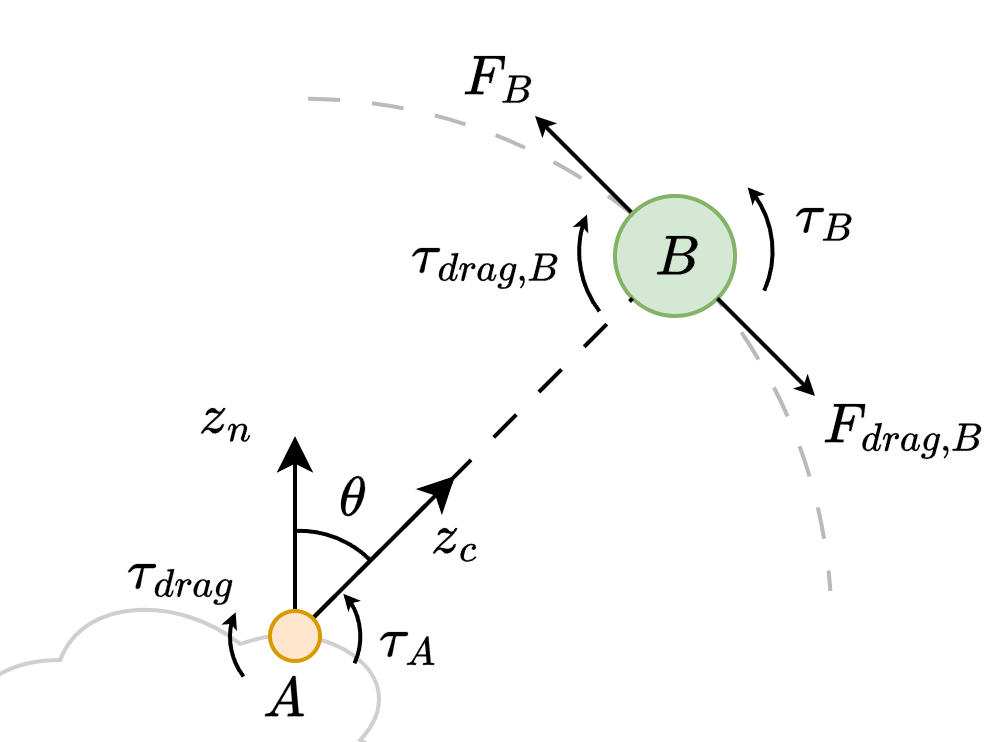
\includegraphics[width=0.55\linewidth]{FBD.png}
\caption{Free-body representation of the virtual sphere used in the admittance model. Point $A$ denotes the pivot associated with the robot end-effector, while point $B$ denotes the center of mass of the virtual sphere. The rotational motion generated about $A$ produces an equivalent force $F_B$ and torque $\tau_B$ at the sphere center, while viscous drag force $F_{\mathrm{drag},B}$ and drag torque $\tau_{\mathrm{drag},B}$ oppose motion.}
\label{fig:virtual_sphere_dynamics}
\end{figure}

\subsubsection{Linear dynamics of the virtual sphere}

Once the angular acceleration $\alpha$ is known, the linear acceleration of the sphere center is obtained as

\begin{equation}
a_B = \alpha d
\end{equation}

where $d$ is the distance between points $A$ and $B$.

Applying Newton's second law to the free body at point $B$ gives

\begin{equation}
F_B = m a_B - F_{\mathrm{drag},B}
\end{equation}

where the translational viscous drag force is

\begin{equation}
F_{\mathrm{drag},B} = -6\pi \mu R v_B.
\end{equation}

Therefore,

\begin{equation}
F_B = m(\alpha d) + 6\pi \mu R v_B.
\end{equation}

\subsubsection{Rotational dynamics of the virtual sphere}

Similarly, applying Euler's rotational equation about the center of mass gives

\begin{equation}
\tau_B = I_B \alpha - \tau_{\mathrm{drag},B}
\end{equation}

where the rotational drag torque is modeled as

\begin{equation}
\tau_{\mathrm{drag},B} = -\gamma \omega_B.
\end{equation}

Thus,

\begin{equation}
\tau_B = I_B \alpha + \gamma \omega_B
\end{equation}

where $I_B = \frac{2}{5}mR^2$ and $\omega_B = \omega_A$.


\subsubsection{Net inputs to the admittance model}

The net force and torque supplied to the admittance model are obtained by subtracting the viscous drag terms from the equivalent free-body quantities:

\begin{equation}
F_{\mathrm{net}} = F_B - 6\pi \mu R v_B
\end{equation}

\begin{equation}
\tau_{\mathrm{net}} = \tau_B - \gamma \omega_B.
\end{equation}

These effective inputs are then used in the admittance dynamics of Section B to generate the commanded translational and rotational velocities of the end-effector.
\section{Experiments and Results}

To validate the proposed orientation control and admittance framework, experiments were conducted using the UR5e manipulator equipped with an eye-in-hand Intel RealSense D405 depth camera. The objective of the experiment is to regulate the end-effector orientation by aligning the camera optical axis with the estimated surface normal obtained from the point cloud.
The experiments were
performed under two different initial error conditions in order
to evaluate the behavior of the controller both within and
beyond the torque saturation region.
 The experimental results were compared with a synthetic MATLAB simulation that emulates the same control pipeline, including the orientation PD controller and the admittance dynamics.
\subsection{Experimental Conditions}
\subsubsection{Small Initial Error Case}

In the first experiment, the initial error was set to $15^\circ$. The saturation threshold was set to $\theta_{max} = 90^\circ$, ensuring that the controller operated entirely in the unsaturated regime.

The parameters used in the experiment were:

\begin{itemize}
\item Initial angle: $15^\circ$
\item Saturation threshold: $\theta_{max} = 90^\circ$
\item Maximum linear velocity: $v_{max} = 0.1\,\mathrm{m/s}$
\item Camera offset from pivot: $d = 0.3\,\mathrm{m}$
\end{itemize}

Under these conditions, the controller operates without torque saturation and the system response is dominated by the nominal admittance dynamics.

\subsubsection{Large Initial Error Case}

In the second experiment, the initial error was increased to $40^\circ$. In this case, the torque saturation threshold was set to $\theta_{max} = 20^\circ$, causing the controller to enter the saturated regime during the initial phase of motion.

The parameters used in this experiment were:

\begin{itemize}
\item Initial angle: $40^\circ$
\item Saturation threshold: $\theta_{max} = 20^\circ$
\item Maximum linear velocity: $v_{max} = 0.1\,\mathrm{m/s}$
\item Camera offset from pivot: $d = 0.3\,\mathrm{m}$
\end{itemize}

When the initial orientation error exceeds $\theta_{max}$, the controller torque saturates at the actuator limit. This results in the end-effector moving initially close to the maximum allowable velocity before transitioning to the nominal admittance-controlled behavior as the orientation error decreases.
% \subsection{Experiment 1: Small Orientation Error ($15^\circ$)}

% In the first experiment, the robot started with an initial orientation error of approximately $15^\circ$. The orientation controller generated torque commands based on the error, which were then passed through the admittance model to produce velocity commands for the robot.

% Fig.~\ref{fig:exp15} shows the angle error evolution over time for both the synthetic simulation and the hardware experiment. The measured hardware trajectory closely follows the simulated response and converges smoothly to zero, indicating stable closed-loop behavior.

% The torque commands generated by the controller are shown in Fig.~\ref{fig:exp15}. The hardware torque commands exhibit similar magnitude and temporal trends as the synthetic simulation, demonstrating that the controller implementation in the ROS2 pipeline behaves consistently with the simulated model.

% The resulting translational velocity along the camera axis $v$ is shown in Fig.~\ref{fig:vel15}. The hardware velocity closely follows the admittance-integrated synthetic velocity, confirming that the velocity commands produced by the controller are faithfully executed by the Servo node.

% Similarly, Fig.~\ref{fig:vel15} shows the angular velocity $\omega$ of the end-effector. The experimental measurements track the synthetic admittance prediction with comparable magnitude and shape. Minor deviations arise due to sensing noise, estimation errors, and internal robot controller dynamics.

% Overall, the results demonstrate that for Small orientation errors, the proposed control architecture produces hardware responses that closely match the simulated admittance dynamics.

% \subsection{Experiment 2: Large Orientation Error ($40^\circ$)}

% A second experiment was conducted with a larger initial error of approximately $40^\circ$ in order to evaluate controller behavior under more aggressive correction requirements.

% Fig.~\ref{fig:exp40} shows the error evolution. Despite the significantly larger initial misalignment, the controller successfully drives the orientation error toward zero while maintaining stable system behavior.

% The torque commands for this experiment are shown in Fig.~\ref{fig:exp40}. In contrast to the Small-error case, the commanded torque initially reaches the actuator saturation limit. This behavior is expected because the large initial error produces a high control effort from the PD controller.

% The saturation of the torque command results in the end-effector moving at the maximum allowable velocity imposed by the controller. This behavior is reflected in the velocity plots.

% Fig.~\ref{fig:vel40} shows the linear velocity $v$, where the hardware velocity closely follows the synthetic admittance model but reaches higher magnitudes compared to the Small-error experiment.

% Similarly, Fig.~\ref{fig:vel40} shows the angular velocity $\omega$. The angular velocity initially reaches a larger magnitude due to the higher torque command, before gradually decreasing as the orientation error converges.

% These results confirm that the controller remains stable even for large initial errors while respecting the torque saturation constraints built into the control design.

% \subsection{Discussion}

% Across both experiments, the synthetic simulation and the hardware measurements show strong agreement in terms of error convergence, velocity trends, and torque commands. Small discrepancies are primarily caused by sensor noise, estimation uncertainty in the normal vector, and the internal dynamics of the robot controller.

% The close correspondence between simulation and hardware validates the accuracy of the proposed admittance-based control framework and demonstrates that the MATLAB simulation provides a reliable representation of the real robot behavior.
% \begin{figure}[t]
% \centering

% \begin{subfigure}{0.95\linewidth}
% \centering
% 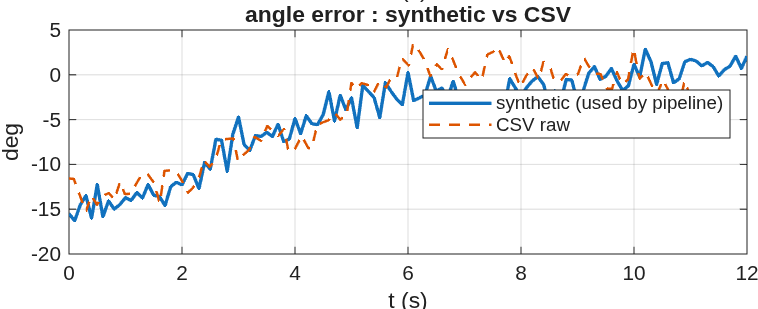
\includegraphics[width=\linewidth]{angleerror15deg.png}
% \caption{angle error for $15^\circ$ initial orientation error.}
% \end{subfigure}

% \vspace{0.3cm}

% \begin{subfigure}{0.95\linewidth}
% \centering
% 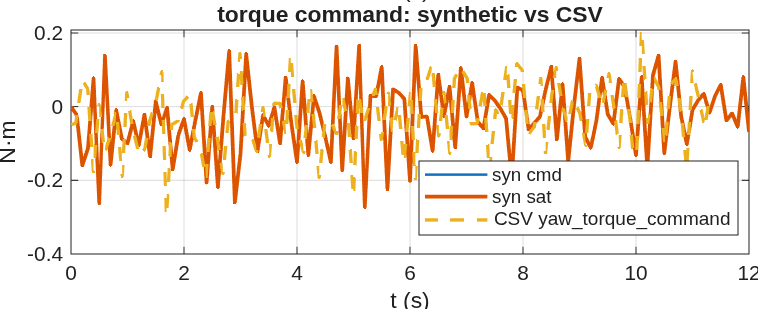
\includegraphics[width=\linewidth]{torque15deg.png}
% \caption{Torque command generated by the controller.}
% \end{subfigure}

% \caption{Controller performance for the $15^\circ$ experiment. The angular error converges to zero while the controller torque remains bounded and follows the same trend as the hardware measurements.}
% \label{fig:exp15}
% \end{figure}
\begin{figure}[t]
\centering
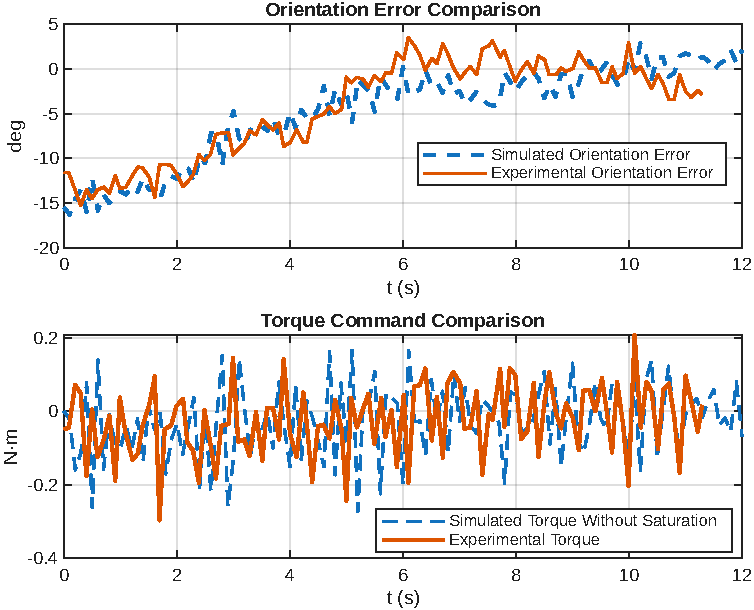
\includegraphics[width=\linewidth]{15degangletorque.pdf}
\caption{Comparison of orientation error and torque command between simulation and experiment for the $15^\circ$ initial orientation error case. The top subplot shows the angle error convergence, while the bottom subplot shows the corresponding torque command generated by the controller. The experimental measurements closely match the simulated controller response. Here since the initial orientation error is smaller than $\theta_{max}$ no saturation is observed in the torque command.}
\label{fig:angle_torque_15}
\end{figure}
% \begin{figure}[t]
% \centering
% \begin{subfigure}{0.48\linewidth}
% \centering
% 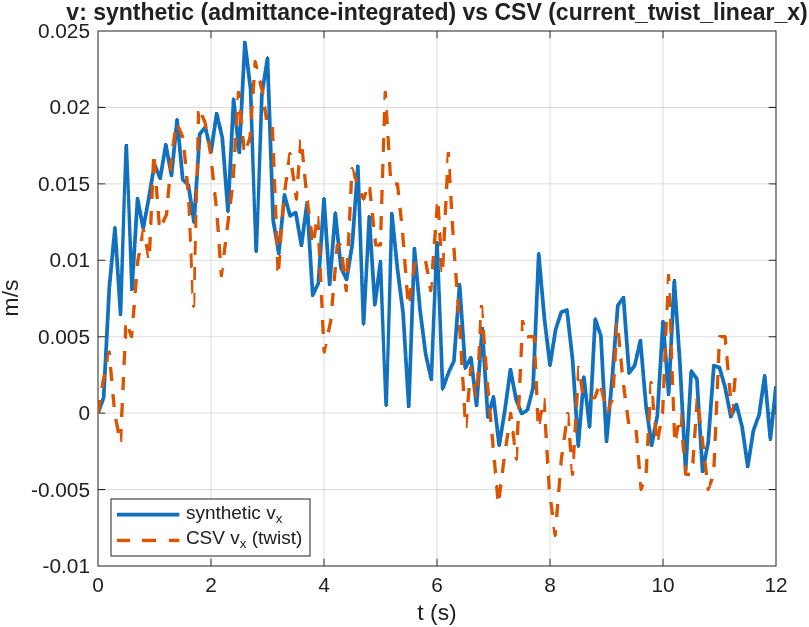
\includegraphics[width=\linewidth]{v15deg.png}
% \caption{Linear velocity $v$ for the $15^\circ$ experiment.}
% \end{subfigure}
% \hfill
% \begin{subfigure}{0.48\linewidth}
% \centering
% 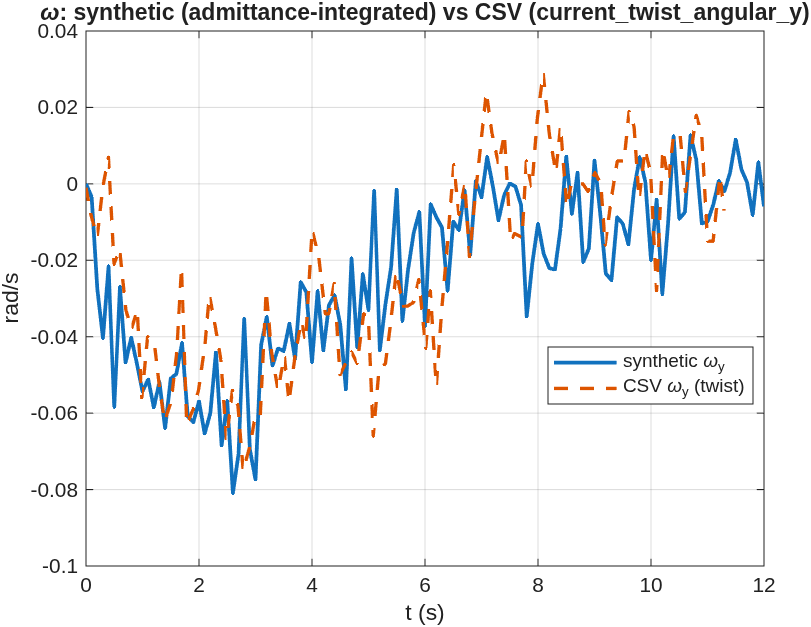
\includegraphics[width=\linewidth]{w15deg.png}
% \caption{Angular velocity $\omega$ for the $15^\circ$ experiment.}
% \end{subfigure}

% \caption{Velocity response of the admittance controller for the $15^\circ$ experiment. 
% The measured velocities closely follow the synthetic admittance predictions.}
% \label{fig:vel15}
% \end{figure}
\begin{figure}[t]
\centering
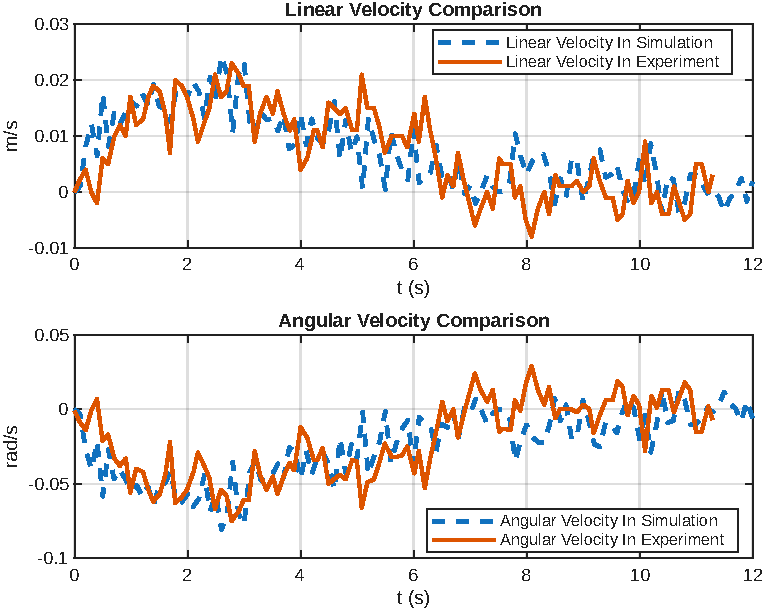
\includegraphics[width=\linewidth]{15degvelandw.pdf}
\caption{Comparison of linear and angular velocities between simulation and experiment for the $15^\circ$ initial orientation error case. The top subplot shows the linear velocity $v$, while the bottom subplot shows the angular velocity $\omega$. The experimental measurements closely follow the velocities predicted by the synthetic admittance model.}
\label{fig:vel15}
\end{figure}
% \begin{figure}[t]
% \centering

% \begin{subfigure}{0.95\linewidth}
% \centering
% 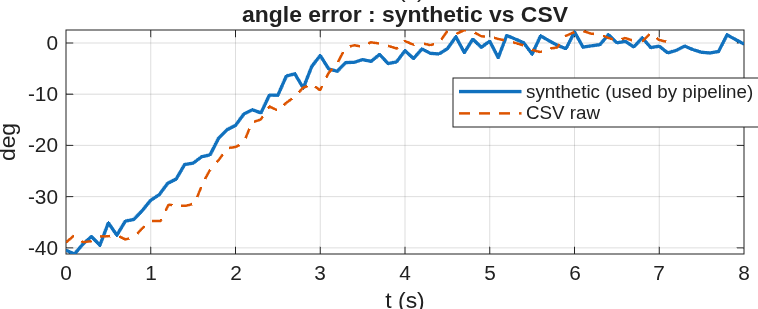
\includegraphics[width=\linewidth]{angle40deg.png}
% \caption{Yaw angle error for $40^\circ$ initial orientation error.}
% \end{subfigure}

% \vspace{0.3cm}

% \begin{subfigure}{0.95\linewidth}
% \centering
% 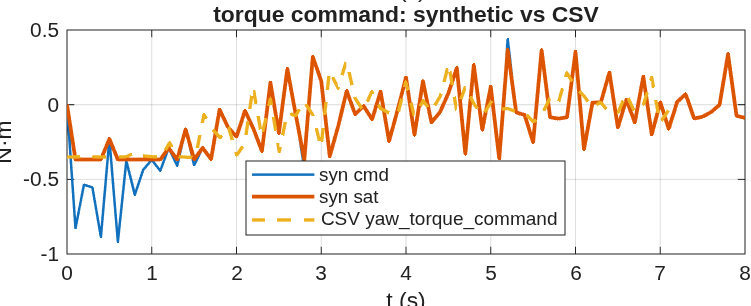
\includegraphics[width=\linewidth]{torque40deg.png}
% \caption{Torque command generated by the controller.}
% \end{subfigure}

% \caption{Controller response for the $40^\circ$ experiment. The larger initial error produces higher torque commands and leads to temporary torque saturation during the initial phase of the motion.}
% \label{fig:exp40}
% \end{figure}
\begin{figure}[t]
\centering
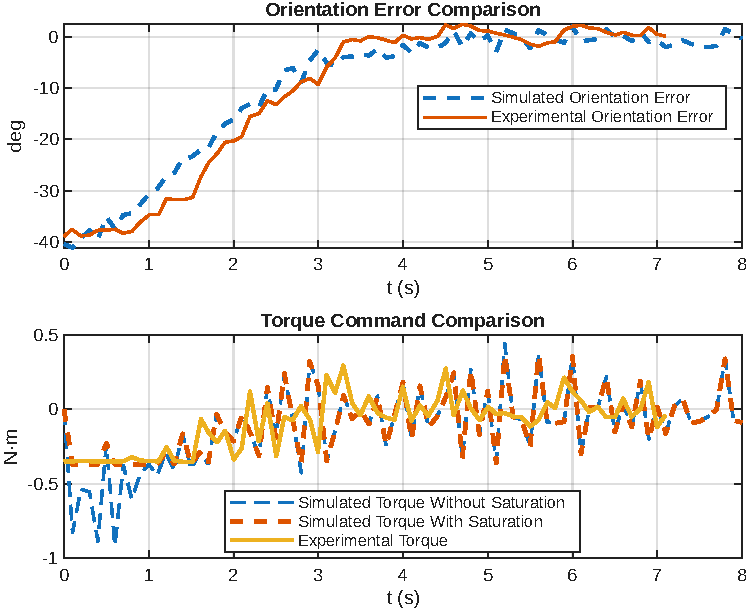
\includegraphics[width=\linewidth]{40degangletorque.pdf}
\caption{Comparison of orientation error and torque command between simulation and experiment for the $40^\circ$ initial orientation error case. The top subplot shows the angle error convergence, while the bottom subplot shows the corresponding torque command generated by the controller. The experimental measurements follow the synthetic controller predictions, with torque saturation occurring during the initial phase due to the large orientation error.}
\label{fig:angle_torque_40}
\end{figure}
% \begin{figure}[t]
% \centering
% \begin{subfigure}{0.48\linewidth}
% \centering
% 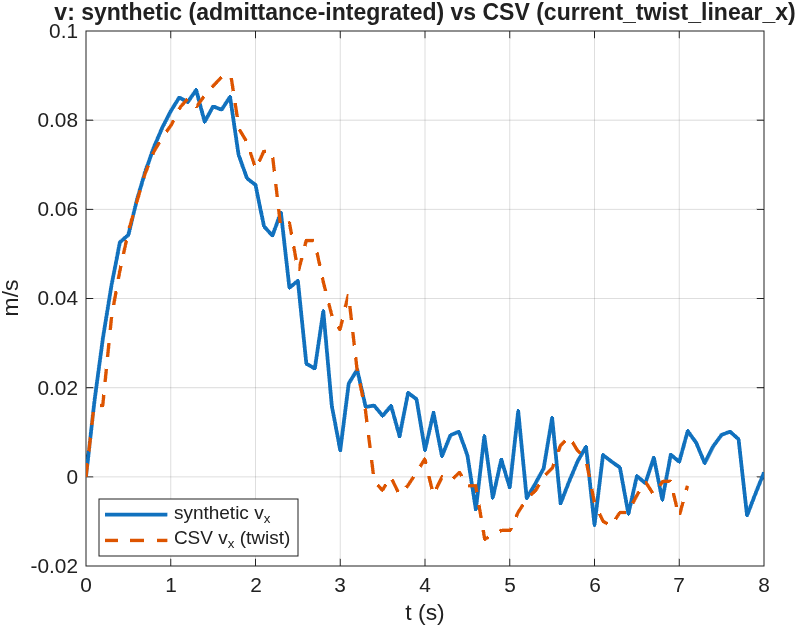
\includegraphics[width=\linewidth]{v40deg.png}
% \caption{Linear velocity $v$ for the $40^\circ$ experiment.}
% \end{subfigure}
% \hfill
% \begin{subfigure}{0.48\linewidth}
% \centering
% 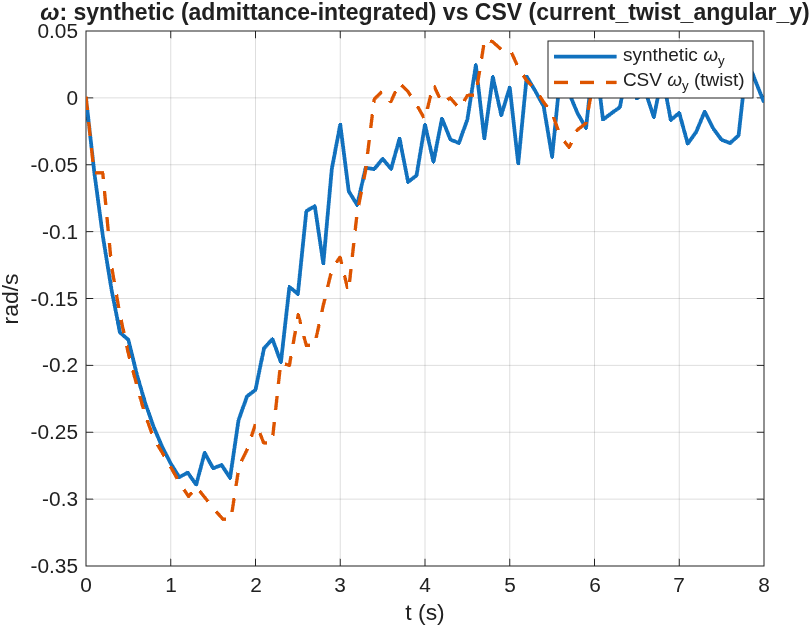
\includegraphics[width=\linewidth]{w40deg.png}
% \caption{Angular velocity $\omega$ for the $40^\circ$ experiment.}
% \end{subfigure}

% \caption{Velocity response of the admittance controller for the $40^\circ$ experiment. 
% Higher velocities are observed due to the larger initial orientation error and increased control effort.}
% \label{fig:vel40}
% \end{figure}
\begin{figure}[t]
\centering
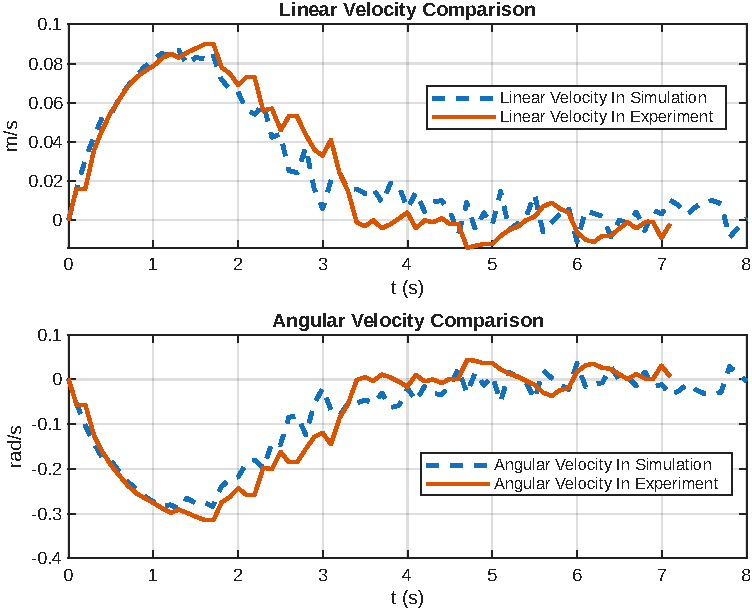
\includegraphics[width=\linewidth]{40degvelandw.pdf}
\caption{Linear and angular velocity comparison between simulation and experiment for the $40^\circ$ initial orientation error case. The top plot shows the linear velocity $v$ while the bottom plot shows the angular velocity $\omega$. The experimental measurements closely follow the synthetic admittance model predictions.}
\label{fig:vel40}
\end{figure}
% \subsection{Validation of Admittance Model Using Synthetic and Hardware Data}

% To validate the accuracy of the proposed admittance control framework, a comparison was performed between the simulated admittance model and experimental data collected from the UR5e manipulator. The objective of this experiment is to verify that the synthetic simulation used in MATLAB accurately reproduces the behavior of the physical system.

% The experiment considers a yaw orientation error case where the controller generates torque commands that are integrated through the admittance model to produce angular and linear velocities. These synthetic outputs are compared against the corresponding quantities recorded from the robot through the ROS2 pipeline.

% \subsubsection{Torque Command Comparison}

% Figure~\ref{fig:torque_validation} compares the torque command generated in simulation with the torque command observed in the real system. The synthetic torque signal represents the commanded torque produced by the PD orientation controller, while the CSV signal corresponds to the torque command recorded during the hardware experiment.

% The results show that the simulated torque closely follows the trend of the experimental torque signal, including the magnitude and frequency characteristics. Minor discrepancies are primarily attributed to sensor noise and discretization effects in the real system.

% \begin{figure}[H]
% \centering
% \includegraphics[width=0.9\linewidth]{torque15degyaw.png.png}
% \caption{Yaw torque command comparison between synthetic simulation and hardware data.}
% \label{fig:torque_validation}
% \end{figure}

% \subsubsection{Angular Velocity Validation}

% The angular velocity produced by the admittance model is compared against the angular velocity measured from the robot twist message. Figure~\ref{fig:omega_validation} shows the comparison between the synthetic angular velocity and the experimentally observed angular velocity.

% The results demonstrate that the angular velocity trends match closely, indicating that the admittance integration used in the simulation accurately captures the dynamic response of the system.

% \begin{figure}[H]
% \centering
% \includegraphics[width=0.9\linewidth]{wy15deg.png}
% \caption{Comparison of angular velocity about the y-axis between the synthetic admittance model and the hardware measurements.}
% \label{fig:omega_validation}
% \end{figure}

% \subsubsection{Linear Velocity Validation}

% The angular velocity generated by the admittance controller is mapped to the linear velocity of the end-effector through the geometric relationship between rotational motion and the camera offset from the pivot point. Figure~\ref{fig:vx_validation} compares the linear velocity predicted by the simulation with the velocity measured from the robot.

% The close agreement between the two signals confirms that the kinematic mapping used in the model correctly captures the relationship between rotational motion and the resulting translational velocity of the inspection camera.

% \begin{figure}[H]
% \centering
% \includegraphics[width=0.9\linewidth]{vx15deg.png}
% \caption{Comparison of linear velocity along the x-axis between synthetic admittance integration and hardware measurements.}
% \label{fig:vx_validation}
% \end{figure}

% Overall, the results indicate strong agreement between the simulated admittance controller and the hardware implementation. This validates the fidelity of the simulation framework and confirms that the admittance model accurately represents the dynamic behavior of the robotic inspection system.
% The proposed controller was validated through both simulation and hardware experiments. Synthetic trajectories were generated in MATLAB using the derived virtual sphere dynamic model and the PD/admittance controller. Hardware experiments were conducted on a UR5e manipulator using the ROS~2 Servo interface. Orientation errors were computed from surface normals estimated using the eye-in-hand depth camera.
% \subsection{Large Orientation Error Case and Torque Saturation}

% To further evaluate the behavior of the controller under large disturbances, an experiment was conducted with an initial yaw error of approximately $40^\circ$. In this case, the commanded control torque exceeds the allowable actuator limit and therefore activates the torque saturation constraint implemented in the controller.

% Figure~\ref{fig:torque_sat} shows the torque command generated by the synthetic model compared with the torque signal recorded from the hardware experiment. The blue curve represents the unsaturated torque command produced by the PD controller, while the red curve represents the saturated torque applied to the system. The hardware torque signal closely follows the saturated command, confirming that the actuator limits enforced in the simulation accurately represent the behavior of the real system.

% \begin{figure}[H]
% \centering
% 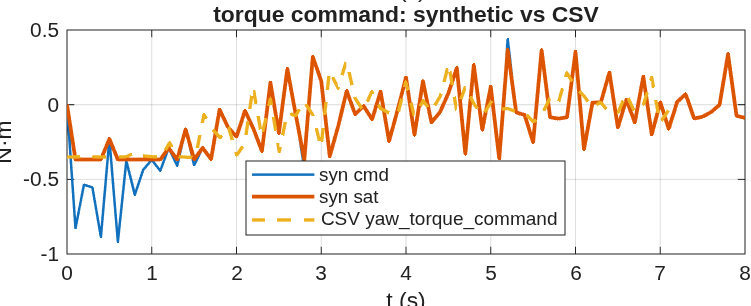
\includegraphics[width=0.9\linewidth]{torque40deg.png}
% \caption{Yaw torque command comparison for the $40^\circ$ initial yaw error case showing actuator torque saturation.}
% \label{fig:torque_sat}
% \end{figure}

% The effect of torque saturation on the angular velocity of the system is shown in Figure~\ref{fig:omega_sat}. Due to the torque limit, the angular acceleration becomes bounded, resulting in a slower dynamic response compared to the smaller-angle experiment. Nevertheless, the synthetic admittance model continues to track the overall trend of the measured angular velocity from the robot.

% \begin{figure}[H]
% \centering
% \includegraphics[width=0.9\linewidth]{wy40deg.png}
% \caption{Angular velocity comparison for the $40^\circ$ initial yaw error case between the synthetic admittance model and hardware measurements.}
% \label{fig:omega_sat}
% \end{figure}

% The corresponding linear velocity of the inspection camera along the $x$ direction is shown in Figure~\ref{fig:vx_sat}. As the torque saturates, the system reaches the maximum allowable velocity determined by the admittance model and the viscous drag constraint used to derive the actuator limits. This results in a plateau-like behavior in the velocity response during the initial phase of motion.

% \begin{figure}[H]
% \centering
% \includegraphics[width=0.9\linewidth]{vx40deg.png}
% \caption{Linear velocity comparison for the $40^\circ$ initial yaw error case showing the effect of torque saturation on the translational motion.}
% \label{fig:vx_sat}
% \end{figure}

% Overall, the results demonstrate that the proposed admittance control framework accurately captures the system behavior even in the presence of actuator saturation. The agreement between the synthetic simulation and the hardware measurements confirms that the dynamic model used in the simulation is representative of the physical robot.
% Several experiments were performed using different initial orientation errors. The results show strong agreement between the synthetic trajectories predicted by the model and the measured responses recorded from the robot. In the Small yaw experiment ($15^\circ$), both the synthetic and measured yaw errors converge smoothly to zero with a monotonic response consistent with the critically damped pole placement used in the controller design.

% For larger initial errors, such as the $40^\circ$ yaw case, the torque command reaches its saturation bound during the initial phase of motion. Under this condition, the robot moves at the maximum allowable velocity $v_{\max}$ determined by the actuator limits. Once the orientation error decreases below the design threshold $\theta_{\max}$, the controller transitions back to the linear PD regime and the motion converges smoothly to the desired orientation.

% Pitch regulation experiments demonstrate similar behavior, with close agreement between the model prediction and hardware response. Although small deviations are present due to perception noise and sensing uncertainty, the overall dynamics remain consistent with the predicted admittance model.

% These results confirm that the proposed virtual sphere admittance framework provides an accurate and practical representation of the robot's orientation dynamics, enabling stable and compliant perception-driven control during inspection tasks.
% \section{Discussion}

% The experimental results demonstrate that the proposed admittance-based orientation controller produces stable and consistent behavior across different initial conditions. In all tested cases, the orientation error converges toward zero while maintaining smooth velocity and torque profiles. This behavior confirms that the virtual sphere dynamics combined with the PD controller provide an effective mechanism for regulating orientation during inspection tasks.

% A key observation from the results is the close agreement between the synthetic trajectories obtained from the admittance-integrated model and the measured data recorded from the robot. The yaw and pitch error plots show similar convergence trends for both signals, indicating that the virtual dynamic model captures the dominant behavior of the physical system. This agreement suggests that the simplified mass–damper representation of the end-effector is sufficient to approximate the real robot dynamics for the purposes of outer-loop orientation regulation.

% % The velocity plots further demonstrate that the commanded velocities generated by the admittance model remain bounded and follow the same overall trends as the velocities observed from the robot. Despite measurement noise and small deviations caused by sensing uncertainty, the hardware response remains consistent with the expected behavior predicted by the model. This indicates that the ROS~2 Servo interface executes the commanded velocities reliably without introducing significant distortion.

% % The torque command plots show that the control effort remains bounded even for relatively large initial orientation errors, such as the $40^\circ$ yaw case. This behavior is consistent with the torque saturation constraint incorporated into the controller design, which limits the maximum allowable control input based on actuator capabilities.
% An additional behavior can be observed in the experiment corresponding to the larger initial yaw angle. When the initial orientation error exceeds the design limit $\theta_{\max}$ used in the torque constraint formulation, the commanded control torque reaches the saturation bound. Under this condition, the controller operates in a torque-limited regime where the applied torque is clipped at $\tau_{\max}$. As a result, the end-effector moves at the maximum admissible velocity $v_{\max}$ determined by the actuator constraints.

% This behavior is consistent with the controller design presented in Section~III, where the torque saturation constraint was used to derive the maximum allowable natural frequency and corresponding controller gains. Once the torque reaches its saturation limit, the resulting motion corresponds to the maximum velocity that the system can safely generate. The experimental results confirm this effect, as the velocity profiles reach the imposed $v_{\max}$ bound during the initial phase of the motion before decreasing as the orientation error falls within the controllable range. This observation validates the practical relevance of the torque constraint analysis and demonstrates that the controller behaves predictably even under large initial orientation errors.

% Across the different experiments, the controller demonstrates robustness to perception noise and varying initial angles. The consistent convergence behavior across yaw and pitch regulation suggests that the proposed framework can generalize to different inspection configurations. These results confirm that the combination of perception-driven error feedback, virtual sphere dynamics, and admittance integration provides a practical and reliable approach for compliant orientation control in robotic inspection tasks.
\section{Discussion}

The experimental results demonstrate that the proposed admittance-based orientation control framework produces stable and consistent behavior across different initial conditions. In all tested cases, the orientation error converges toward zero while maintaining smooth velocity and torque profiles. This confirms that the virtual sphere dynamics combined with the PD orientation controller provide an effective mechanism for regulating end-effector orientation during robotic inspection tasks.

A key observation from the results is the close agreement between the synthetic trajectories obtained from the admittance-integrated simulation and the measurements recorded from the robot. The angular error, angular velocity, linear velocity, torque command signals exhibit similar trends in both the simulation and hardware data, as illustrated in Fig.~\ref{fig:angle_torque_15}, Fig.~\ref{fig:vel15}, Fig.~\ref{fig:angle_torque_40} and Fig.~\ref{fig:vel40}. Minor discrepancies are primarily attributed to sensor noise, uncertainty in surface normal estimation, and the internal dynamics of the robot controller. Nevertheless, the overall agreement indicates that the simplified mass–damper representation used in the admittance model captures the dominant behavior of the physical system.

An additional behavior is observed in the experiment corresponding to the larger initial angle. When the initial orientation error exceeds the design limit $\theta_{\max}$ used in the torque constraint formulation, the commanded torque reaches the saturation bound $\tau_{\max}$, as seen in Fig.~\ref{fig:angle_torque_40}. Under this condition, the controller operates in a torque-limited regime where the applied torque is clipped at the actuator limit. As a result, the end-effector initially moves at the maximum admissible velocity $v_{\max}$ determined by the actuator constraints.

This behavior is further reflected in the velocity profiles shown in Fig.~\ref{fig:vel40}, where the linear velocity reaches the imposed $v_{\max}$ bound during the initial phase of motion before decreasing as the orientation error falls within the controllable range. This observation is consistent with the controller design presented earlier, where the torque saturation constraint was used to derive the maximum allowable system response.

Overall, the controller demonstrates robustness to perception noise and varying initial orientation errors and validates the proposed admittance-based control framework, indicating that the MATLAB simulation provides a reliable representation of the real robot dynamics.

\section{Future Work}

An important direction for future work is extending the proposed framework to support the fusion of multiple control objectives within a unified dynamic structure. Admittance control provides a natural interface for such integration, as it maps generalized wrench or interaction objectives into motion commands.

Through this formulation, perception-driven orientation corrections, operator teleoperation inputs, and disturbance rejection mechanisms can be expressed as equivalent inputs to the same admittance dynamics. Additional sensing objectives, such as autofocus control, can also be incorporated within this framework. This enables multiple control objectives to be combined without modifying the underlying robot servo architecture.

A promising extension of this work is the development of an operator-assisted inspection system where teleoperation inputs provide coarse positioning while the perception-driven controller performs automatic orientation alignment using estimated surface normals. Future research will also investigate the use of PID-based controllers within this framework to reduce tracking error during teleoperation and regulate interaction dynamics when multiple control objectives are present, enabling more flexible and adaptive robotic inspection.


% An example of a floating figure using the graphicx package.
% Note that \label must occur AFTER (or within) \caption.
% For figures, \caption should occur after the \includegraphics.
% Note that IEEEtran v1.7 and later has special internal code that
% is designed to preserve the operation of \label within \caption
% even when the captionsoff option is in effect. However, because
% of issues like this, it may be the safest practice to put all your
% \label just after \caption rather than within \caption{}.
%
% Reminder: the "draftcls" or "draftclsnofoot", not "draft", class
% option should be used if it is desired that the figures are to be
% displayed while in draft mode.
%
%\begin{figure}[!t]
%\centering
%\includegraphics[width=2.5in]{myfigure}
% where an .eps filename suffix will be assumed under latex, 
% and a .pdf suffix will be assumed for pdflatex; or what has been declared
% via \DeclareGraphicsExtensions.
%\caption{Simulation results for the network.}
%\label{fig_sim}
%\end{figure}

% Note that the IEEE typically puts floats only at the top, even when this
% results in a large percentage of a column being occupied by floats.


% An example of a double column floating figure using two subfigures.
% (The subfig.sty package must be loaded for this to work.)
% The subfigure \label commands are set within each subfloat command,
% and the \label for the overall figure must come after \caption.
% \hfil is used as a separator to get equal spacing.
% Watch out that the combined width of all the subfigures on a 
% line do not exceed the text width or a line break will occur.
%
%\begin{figure*}[!t]
%\centering
%\subfloat[Case I]{\includegraphics[width=2.5in]{box}%
%\label{fig_first_case}}
%\hfil
%\subfloat[Case II]{\includegraphics[width=2.5in]{box}%
%\label{fig_second_case}}
%\caption{Simulation results for the network.}
%\label{fig_sim}
%\end{figure*}
%
% Note that often IEEE papers with subfigures do not employ subfigure
% captions (using the optional argument to \subfloat[]), but instead will
% reference/describe all of them (a), (b), etc., within the main caption.
% Be aware that for subfig.sty to generate the (a), (b), etc., subfigure
% labels, the optional argument to \subfloat must be present. If a
% subcaption is not desired, just leave its contents blank,
% e.g., \subfloat[].


% An example of a floating table. Note that, for IEEE style tables, the
% \caption command should come BEFORE the table and, given that table
% captions serve much like titles, are usually capitalized except for words
% such as a, an, and, as, at, but, by, for, in, nor, of, on, or, the, to
% and up, which are usually not capitalized unless they are the first or
% last word of the caption. Table text will default to \footnotesize as
% the IEEE normally uses this smaller font for tables.
% The \label must come after \caption as always.
%
%\begin{table}[!t]
%% increase table row spacing, adjust to taste
%\renewcommand{\arraystretch}{1.3}
% if using array.sty, it might be a good idea to tweak the value of
% \extrarowheight as needed to properly center the text within the cells
%\caption{An Example of a Table}
%\label{table_example}
%\centering
%% Some packages, such as MDW tools, offer better commands for making tables
%% than the plain LaTeX2e tabular which is used here.
%\begin{tabular}{|c||c|}
%\hline
%One & Two\\
%\hline
%Three & Four\\
%\hline
%\end{tabular}
%\end{table}


% Note that the IEEE does not put floats in the very first column
% - or typically anywhere on the first page for that matter. Also,
% in-text middle ("here") positioning is typically not used, but it
% is allowed and encouraged for Computer Society conferences (but
% not Computer Society journals). Most IEEE journals/conferences use
% top floats exclusively. 
% Note that, LaTeX2e, unlike IEEE journals/conferences, places
% footnotes above bottom floats. This can be corrected via the
% \fnbelowfloat command of the stfloats package.





\section{Conclusion}

This paper presented an admittance-based orientation control framework for perception-driven robotic visual inspection. The method models the manipulator end-effector as a virtual sphere moving in a viscous medium, resulting in a physically interpretable mass–damper system that generates compliant motion from orientation error. Surface normals estimated from depth point clouds provide real-time orientation feedback, while a PD controller generates the virtual control torque that drives the virtual dynamics. The resulting velocity commands are converted into joint-level commands through inverse kinematics and executed by the robot’s existing servo architecture, allowing the controller to function as a modular outer-loop layer.

Experimental validation on a UR5e manipulator equipped with an eye-in-hand Intel RealSense D405 camera demonstrates stable orientation regulation under varying initial conditions and perception uncertainty. The results show a strong agreement between the model predictions and the hardware response, with bounded torque and velocity profiles consistent with the controller design. The proposed framework therefore provides a practical approach for integrating perception-driven control with existing robotic servo systems for inspection applications.




% if have a single appendix:
%\appendix[Proof of the Zonklar Equations]
% or
%\appendix  % for no appendix heading
% do not use \section anymore after \appendix, only \section*
% is possibly needed

% use appendices with more than one appendix
% then use \section to start each appendix
% you must declare a \section before using any
% \subsection or using \label (\appendices by itself
% starts a section numbered zero.)
%


% \appendices
% \section{Proof of the First Zonklar Equation}
% Appendix one text goes here.

% you can choose not to have a title for an appendix
% if you want by leaving the argument blank
% \section{}
% Appendix two text goes here.


% use section* for acknowledgment
% \section*{Acknowledgment}


% The authors would like to thank...


% Can use something like this to put references on a page
% by themselves when using endfloat and the captionsoff option.
% \ifCLASSOPTIONcaptionsoff
%   \newpage
% \fi



% trigger a \newpage just before the given reference
% number - used to balance the columns on the last page
% adjust value as needed - may need to be readjusted if
% the document is modified later
%\IEEEtriggeratref{8}
% The "triggered" command can be changed if desired:
%\IEEEtriggercmd{\enlargethispage{-5in}}

% references section

% can use a bibliography generated by BibTeX as a .bbl file
% BibTeX documentation can be easily obtained at:
% http://mirror.ctan.org/biblio/bibtex/contrib/doc/
% The IEEEtran BibTeX style support page is at:
% http://www.michaelshell.org/tex/ieeetran/bibtex/
\bibliographystyle{IEEEtran} % TODO: Uncomment these
% argument is your BibTeX string definitions and bibliography database(s)
 \bibliography{references} % TODO: Uncomment these
%
% <OR> manually copy in the resultant .bbl file
% set second argument of \begin to the number of references
% (used to reserve space for the reference number labels box)
%\begin{thebibliography}{1}
% \begin{thebibliography}{99}

% \bibitem{Whitney1977}
% D. E. Whitney,
% ``Force Feedback Control of Manipulator Fine Motions,''
% \emph{Journal of Dynamic Systems, Measurement, and Control},
% vol. 99, no. 2, pp. 91--97, 1977.
% \bibitem{RaibertCraig1981}
% M. H. Raibert and J. J. Craig,
% ``Hybrid Position/Force Control of Manipulators,''
% \emph{Journal of Dynamic Systems, Measurement, and Control},
% vol. 103, no. 2, pp. 126--133, 1981.
% \bibitem{Hogan1985}
% N. Hogan,
% ``Impedance Control: An Approach to Manipulation,''
% \emph{Journal of Dynamic Systems, Measurement, and Control},
% vol. 107, no. 1, pp. 1--24, 1985.

% \bibitem{Maples1986}
% J. A. Maples and J. J. Becker,
% ``Experiments in Force Control of Robotic Manipulators,''
% in \emph{Proceedings of the IEEE International Conference on Robotics and Automation},
% pp. 695--702, 1986.

% \bibitem{Newman1992}
% W. S. Newman,
% ``Stability and Performance Limits of Interaction Controllers,''
% \emph{Journal of Dynamic Systems, Measurement, and Control},
% vol. 114, pp. 563--570, 1992.

% \bibitem{Peshkin1992}
% .~M. Schimmels and M.~A. Peshkin,
% ``The Robustness of an Admittance Control Law Designed for Force-Guided Assembly to the Disturbance of Contact Friction,''
% in \emph{Proceedings of the IEEE International Conference on Robotics and Automation},
% 1992.

% \bibitem{Adams1999}
% R. J. Adams and B. Hannaford,
% ``Stable Haptic Interaction with Virtual Environments,''
% \emph{IEEE Transactions on Robotics and Automation},
% vol. 15, no. 3, pp. 465--474, 1999.

% \bibitem{Duchaine2007}
% V. Duchaine and C. Gosselin,
% ``General Model of Human-Robot Cooperation Using a Velocity-Based Variable Impedance Control,''
% in \emph{Second Joint EuroHaptics Conference and Symposium on Haptic Interfaces for Virtual Environment and Teleoperator Systems},
% pp. 446--451, 2007.
% \bibitem{Keemink2018}
% A. Q. L. Keemink, H. van der Kooij, and A. H. A. Stienen,
% ``Admittance control for physical human–robot interaction,''
% \emph{International Journal of Robotics Research},
% vol. 37, no. 11, pp. 1421--1444, 2018.
% \bibitem{Nandagopal2024}
% A. Nandagopal, A. Kulkarni, C. Acton, K. Manohar, and X. Chen,
% ``Agile Surface Inspection Framework for Aerospace Components Using Unsupervised Machine Learning,''
% in \emph{Proceedings of the International Symposium on Flexible Automation (ISFA)},
% 2024.

% \end{thebibliography}

% biography section
% 
% If you have an EPS/PDF photo (graphicx package needed) extra braces are
% needed around the contents of the optional argument to biography to prevent
% the LaTeX parser from getting confused when it sees the complicated
% \includegraphics command within an optional argument. (You could create
% your own custom macro containing the \includegraphics command to make things
% simpler here.)
%\begin{IEEEbiography}[{\includegraphics[width=1in,height=1.25in,clip,keepaspectratio]{mshell}}]{Michael Shell}
% or if you just want to reserve a space for a photo:

% \begin{IEEEbiography}{Michael Shell}
% Biography text here.
% \end{IEEEbiography}

% % if you will not have a photo at all:
% \begin{IEEEbiographynophoto}{John Doe}
% Biography text here.
% \end{IEEEbiographynophoto}

% % insert where needed to balance the two columns on the last page with
% % biographies
% %\newpage

% \begin{IEEEbiographynophoto}{Jane Doe}
% Biography text here.
% \end{IEEEbiographynophoto}

% You can push biographies down or up by placing
% a \vfill before or after them. The appropriate
% use of \vfill depends on what kind of text is
% on the last page and whether or not the columns
% are being equalized.

%\vfill

% Can be used to pull up biographies so that the bottom of the last one
% is flush with the other column.
%\enlargethispage{-5in}



% that's all folks
\end{document}


